\graphicspath{{chapters/02/images/}}
\chapter{Proteins' geometry}

\section{Introduction}
The study of the geometry of proteins involve what can be learned from protein's coordinates.

\section{The peptide bond}
A protein is a collection of amino acids linked together by a peptide bond.
A carboxylic end and an amino end of two amino acid react together losing a water molecule and forming a peptide bond.
Beside the $\alpha$-carbon there is another one bonded to the oxygen in the carboxylic group and a nitrogen bond in the amino group.
The $\alpha$ carbon is linked to the nitrogen in the amino group of another amino acid.
The carbon and nitrogen display $sp2$ hybridization, the central atom and the $3$ that form a bond with it form a plane, so the peptide bond is planar.
A plane of the peptide bond is formed and rotation of the plane is allowed only around one axis.
\begin{figure}[H]
	\centering
	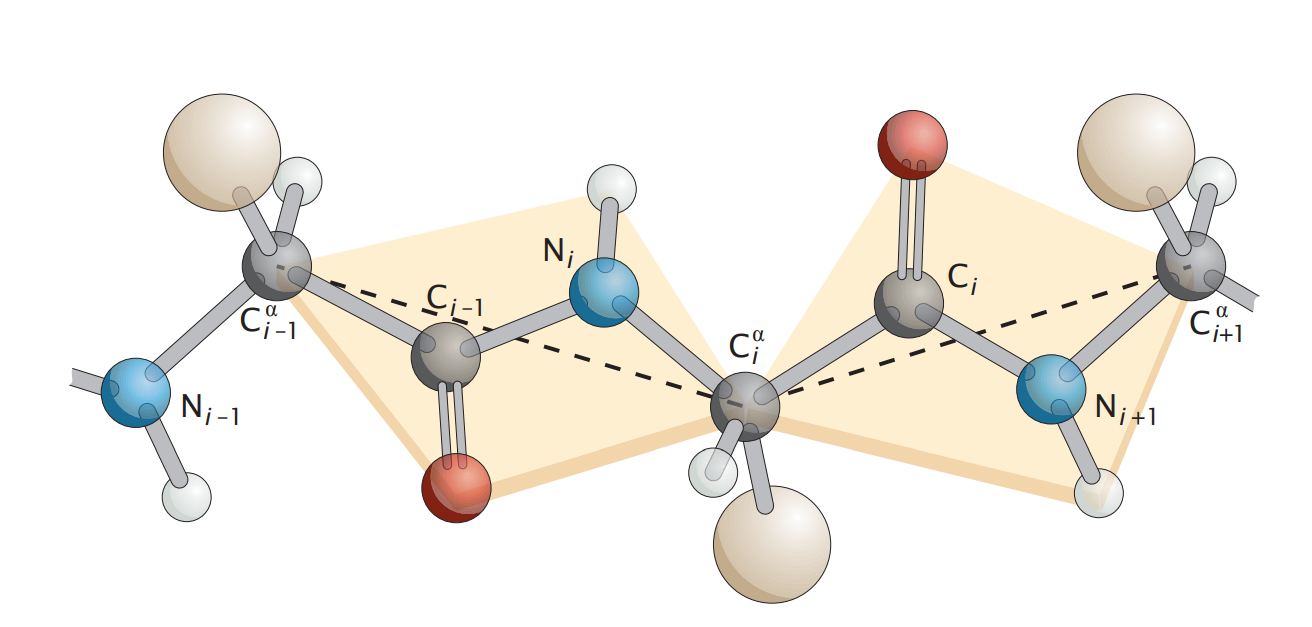
\includegraphics[width=\textwidth]{planar.png}
	\caption{sp2 hybridization of backbone C and N (not $C^{\alpha}$). This is an experimental finding which needs to be incorporated into the system: in this way (and by taking into consideration all the knowledge on proteins), the degree of freedom of the system can be reduced.}
	\label{fig:planar}
\end{figure}

	\subsection{Trans and cis}
	Looking at the peptide bond the carbon atom of the carboxylic group $C'$ and the nitrogen $N$ are each bonded to a different $\alpha$-$C$ and a trans or cis conformation can happen.
	Trying to visualize the atoms that belong to the molecules these repel through the Van der Waals interactions, that can be computed through the Lennard-Jones potential (represented in figure \ref{fig:potential}):

	$$U_{Lj}(r) = E_0\biggl[\biggl(\frac{r_0}{r}\biggr)^{12}-2\biggl(\frac{r_0}{r}\biggr)^6\biggr]$$

	Where:

	\begin{multicols}{2}
		\begin{itemize}
			\item $r_0$ is the distance where the energy is minimum.
			\item $r$ is the distance between two atoms.
			\item $r_{min}$ is the distance at which the energy becomes high.
		\end{itemize}
	\end{multicols}

	\begin{figure}[H]

		\centering
		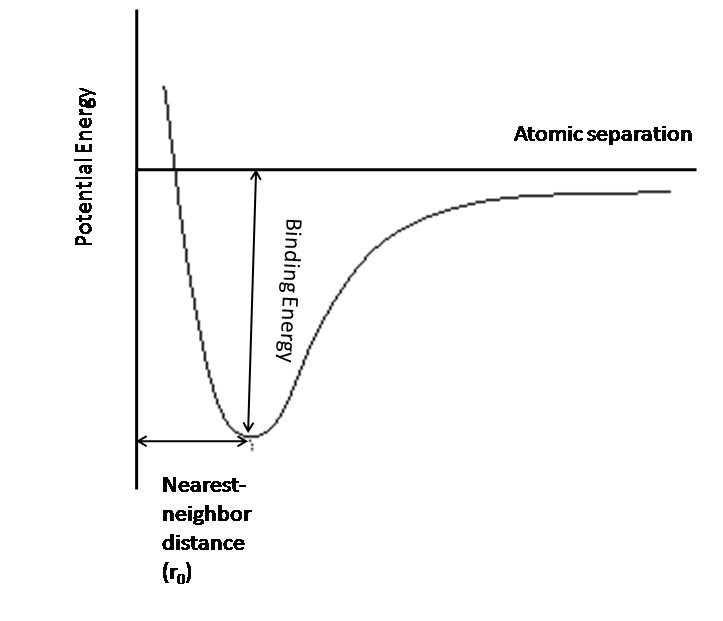
\includegraphics[width=0.5\textwidth]{potential.png}
		\caption{Graphical representation of the energy plotted along the distance between atoms. $r_0$ is the equilibrium distance and it explains the reason why the trans configuration is preferred over the cis configuration}
		\label{fig:potential}
	\end{figure}

	With atoms most of the time the distance between them will be close to $r_0$.
	When decreasing the distance a lot of energy is needed and strain is introduced in the molecule.
	Plotting the values for the energy, $r_0$ and $r_{min}$ the expected distance for each couple of atoms can be seen.
	Focusing on the $C$-$C$ interaction:

	\begin{multicols}{2}
		\begin{itemize}
			\item $r_0 = 3.4\si{\angstrom}$.
			\item $r_{min} = 3.0\si{\angstrom}$.
		\end{itemize}
	\end{multicols}

	When two carbons atoms are below the minimum value the conformation is strained.
	Looking back at the conformation of the peptide bond it can be seen that the cis conformation creates a distance of $2.8\si{\angstrom}$ between the two $\alpha$-$C$, so it is not favourable.
	So the trans conformation is the least energy-hungry and the most present.

	Note that the Lennard-Jones potential is not the only one possible.
	Although it is preferred in most scenarios, other types of potential (e.g., buckingham potential or LJ with different powers) there exist.

\section{The Ramachandran angles}
The planes formed by the peptide bonds can rotate with respect to each other.
So the Ramachandran angles $\phi$ and $\psi$ can be defined between these planes.
For each $\alpha$-$C$:

\begin{multicols}{2}
	\begin{itemize}
		\item $\phi$ describes the rotation around its bond with the nitrogen.
		\item $\psi$ describes the rotation around its bond with the carboxylic group.
	\end{itemize}
\end{multicols}

These are the angles between the subsequent planes.
Some of the angles will require more energy.

	\subsection{Difficulty of rotation}
	It can be seen how a rotation of the $\phi$ angle could cause the two $C'$ to come at a distance of $2.9\si{\angstrom}$ (where $r_{min} = 3.0\si{\angstrom}$.
	On the other hand a rotation of the $\psi$ angle could cause the two $N$ to come at the same distance, but in this case $r_{min}(N-N) = 2.7\si{\angstrom}$.
	In the case of carbon atoms the distance is less than the minimum distance, while in the case of nitrogen it is greater than the minimum allowed value.
	Looking at this it can be seen how the $\psi$ rotation is easier.

	\subsection{Ramachandran plot}
	A Ramachandran plot is a map with the $\phi$ angle on the $x$ axis and the $\psi$ angle on the $y$ axis.
	Because a rotation along the $\phi$ angle is highly disfavoured the angle $0$ is strongly disfavoured and is represented like a black stripe (disallowed region).
	If the amino acids where composed only by carbon and nitrogen atom the Ramachandran map would be the one represented in figure \ref{fig:rama}, where it can be found:

	\begin{multicols}{2}
		\begin{itemize}
			\item A forbidden region in the middle.
			\item Some strained region like for $\psi=0$.
		\end{itemize}
	\end{multicols}

	\begin{figure}[H]
		\centering
		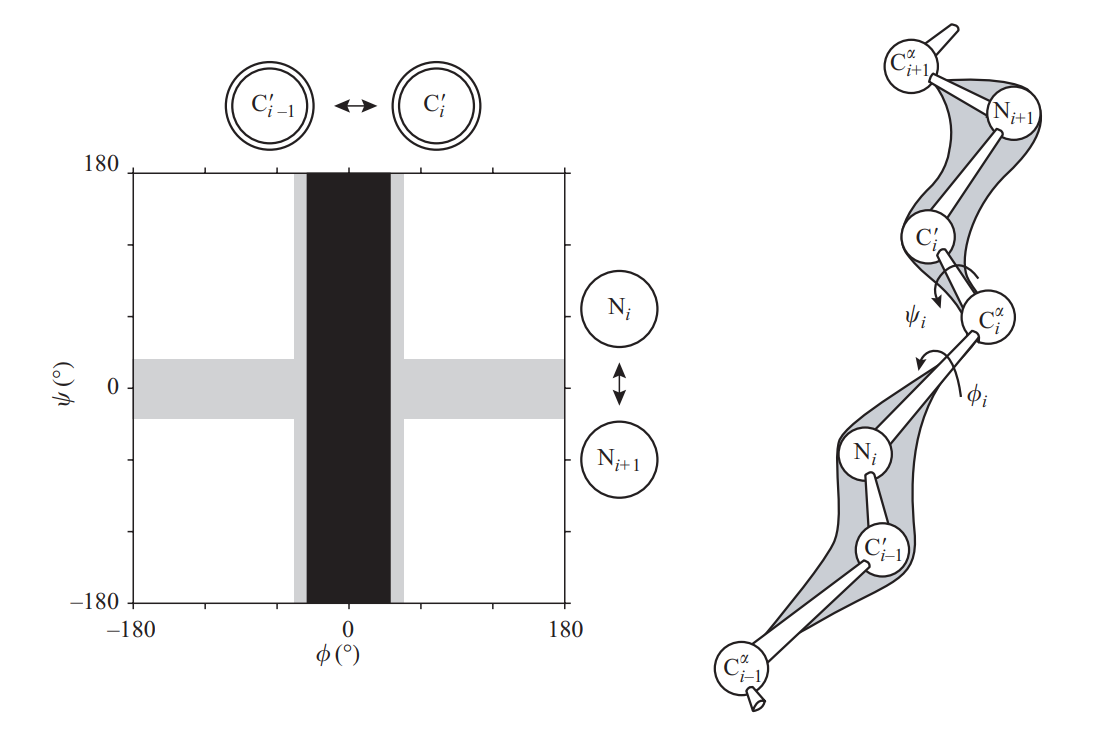
\includegraphics[scale = 0.3]{rama_map.png}
		\caption{This is how Ramachandran plots of the disallowed (black stripe), strained (grey stripe), and fully allowed (white regions) ($\phi$, $\psi$) conformations of the fragment $C^{\alpha}C'N$---$C^{\alpha}$---$C'N-C^{\alpha}$ would look, provided all these atoms had no other atoms attached (right) and atoms of residues $i-1$ and $i+1$ had no interactions.}
		\label{fig:rama}
	\end{figure}

	Looking at a real protein the complexity is increased and the other oxygen and nitrogen atoms are included \ref{fig:ramachandran-complex} and other regions become disallowed due to steady clashes.
	It can be seen how the regions are quite complex.

	\begin{figure}[H]
		\centering
		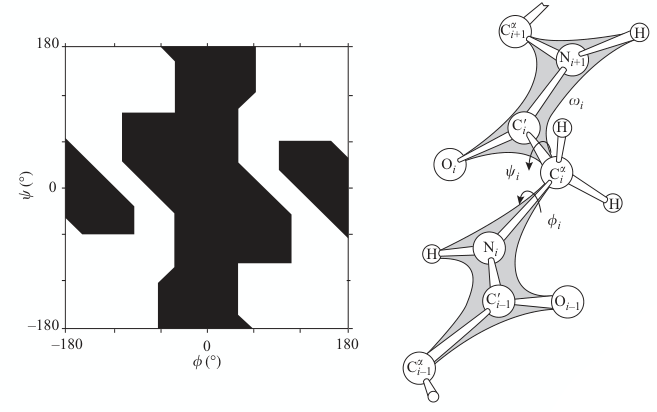
\includegraphics[scale = 0.3]{ramachandran-complex.png}
		\caption{Ramachandran plot of a peptide bond with other atoms.}
		\label{fig:ramachandran-complex}
	\end{figure}

		Looking at a glycine and alanine complex it can be seen in \ref{fig:ala_gly-theo} the space becomes even more complex.

	\begin{figure}[H]
		\centering
		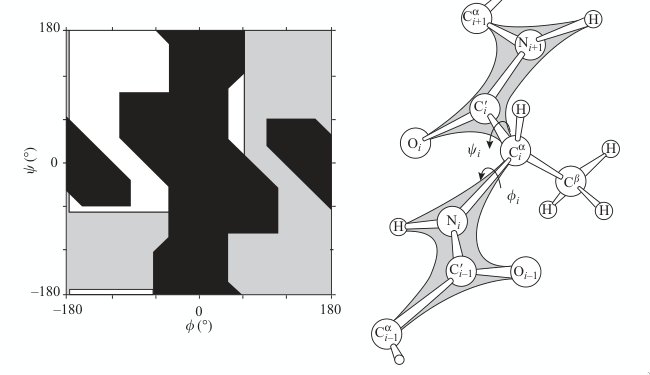
\includegraphics[scale = 0.3]{ala-gly-theo.png}
		\caption{Theoretical representation of a Ramachandran plot of a glycine-alanine complex.}
		\label{fig:ala_gly-theo}
	\end{figure}

	In this case the white regions is very small and a strained region can be seen and the black one.
	Including other residues the allowed region reduces \ref{fig:ramachandran-final}.
	This is due to the presence of larger residues.

	\begin{figure}[H]
		\centering
		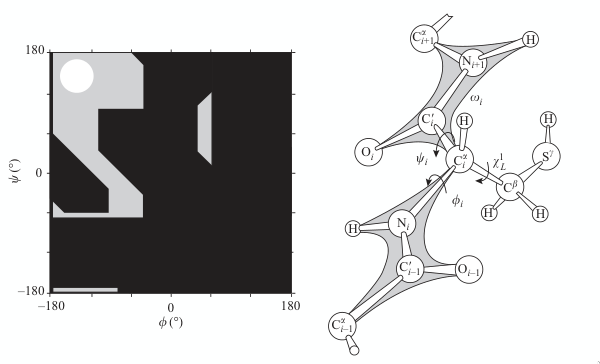
\includegraphics[scale = 0.3]{ramachandran-final.png}
		\caption{Ramachandran plot of a larger residue.}
		\label{fig:ramachandran-final}
	\end{figure}

		\subsubsection{Observed Ramachandran plot}
		Trying to plot for each amino acid its angles an amino acid is represented as a dot.
		Most of the points fall inside of the allowed regions but there are some outliers.
		In some conformation the protein forces the amino acid to assume strange conformations.
		This is done to check if the structure places the amino acids in a proper way.
		A typical observed Ramachandran plot looks like the one in \ref{fig:ala_gly}.

		\begin{figure}[H]
			\centering
			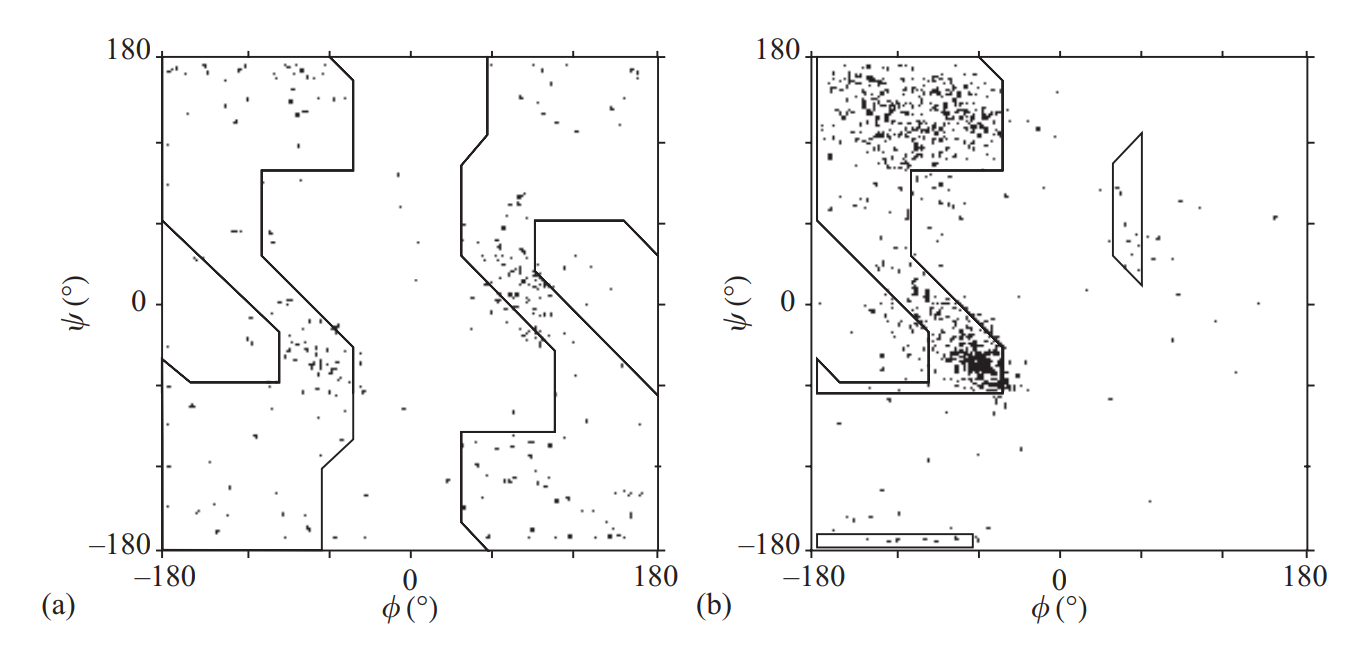
\includegraphics[width=\textwidth]{ala_gly.png}
			\caption{Observed conformations (dots) of glycine (a) and of other amino acid residues (b) in proteins. The sterically allowed regions are contoured.}
			\label{fig:ala_gly}
		\end{figure}


\section{Contact map of proteins}
Starting from the coordinates a contact map can be built.
It is a matrix that map all the contact between the amino acids.
A primary structure can be represented as a collection of beads which will be in contact in the 3D structure.
A square matrix can be built such that each entry in the matrix will determine whether there is a contact or not.
This matrix will be symmetric with diagonal elements with value $1$ and two parallel diagonals for the neighbouring amino acids (figure \ref{fig:contact}).
Secondary structures will have specific signatures:

\begin{multicols}{2}
	\begin{itemize}
		\item $\alpha$-helices: is usually represented by a line parallel to the diagonal.
			This is because the amino acids $i$ is interacting with $i+4$.
		\item $\beta$-strands: the situation is complicated.
			For parallel $\beta$ sheets can be parallel to the diagonal.
			For anti-parallel it can be anti-parallel to the diagonal.
	\end{itemize}
\end{multicols}


\begin{figure}[H]
			\centering
			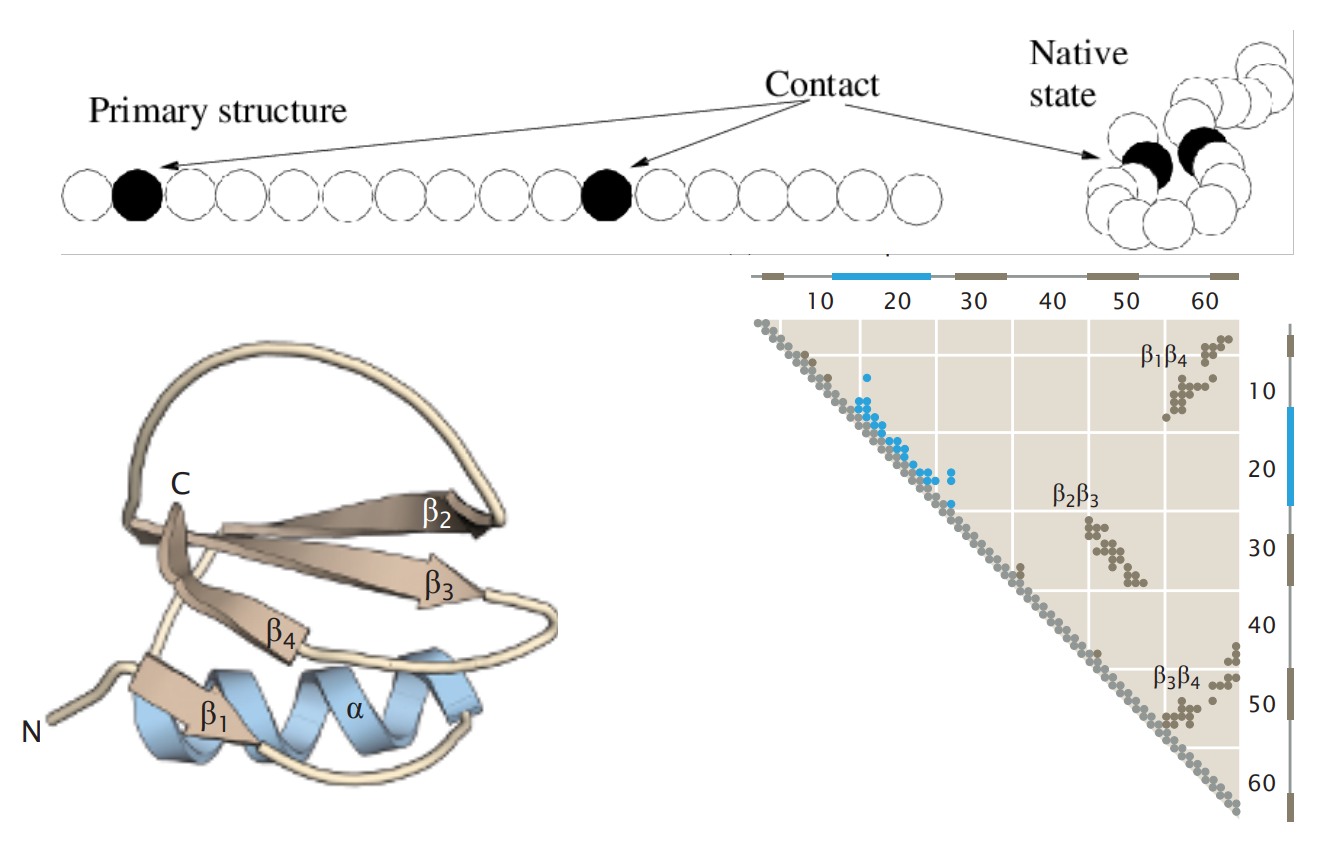
\includegraphics[width=\textwidth]{contact.png}
			\caption{Example of a contact map for a protein.}
			\label{fig:contact}
			\end{figure}


	\subsection{Defining a contact}
	The contact between two amino acids needs to be defined.
	To do so the distance between $\alpha$-$C$ or the distance between the tail of the residue and an $\alpha$-$C$.
	There is also the need to make a trade-off between computational speed and cost.
	Also the dimension of the protein need to be considered when choosing the distance.

\section{Topology diagram}
Having found the secondary structures with a contact map a topology diagram help to understand how those interact with each other (figure \ref{fig:topology}).
In a topology diagram the start is the $N$ terminus and the end the $C$ terminus.
$\beta$-strands are represented as arrows.
If the strands always change direction they will form an anti-parallel $\beta$-sheet.
$\alpha$-helices are represented as small cylinder.
Usually color codes represent the nature of the structure.
This helps with numbering of the secondary structures.

\begin{figure}[H]
			\centering
			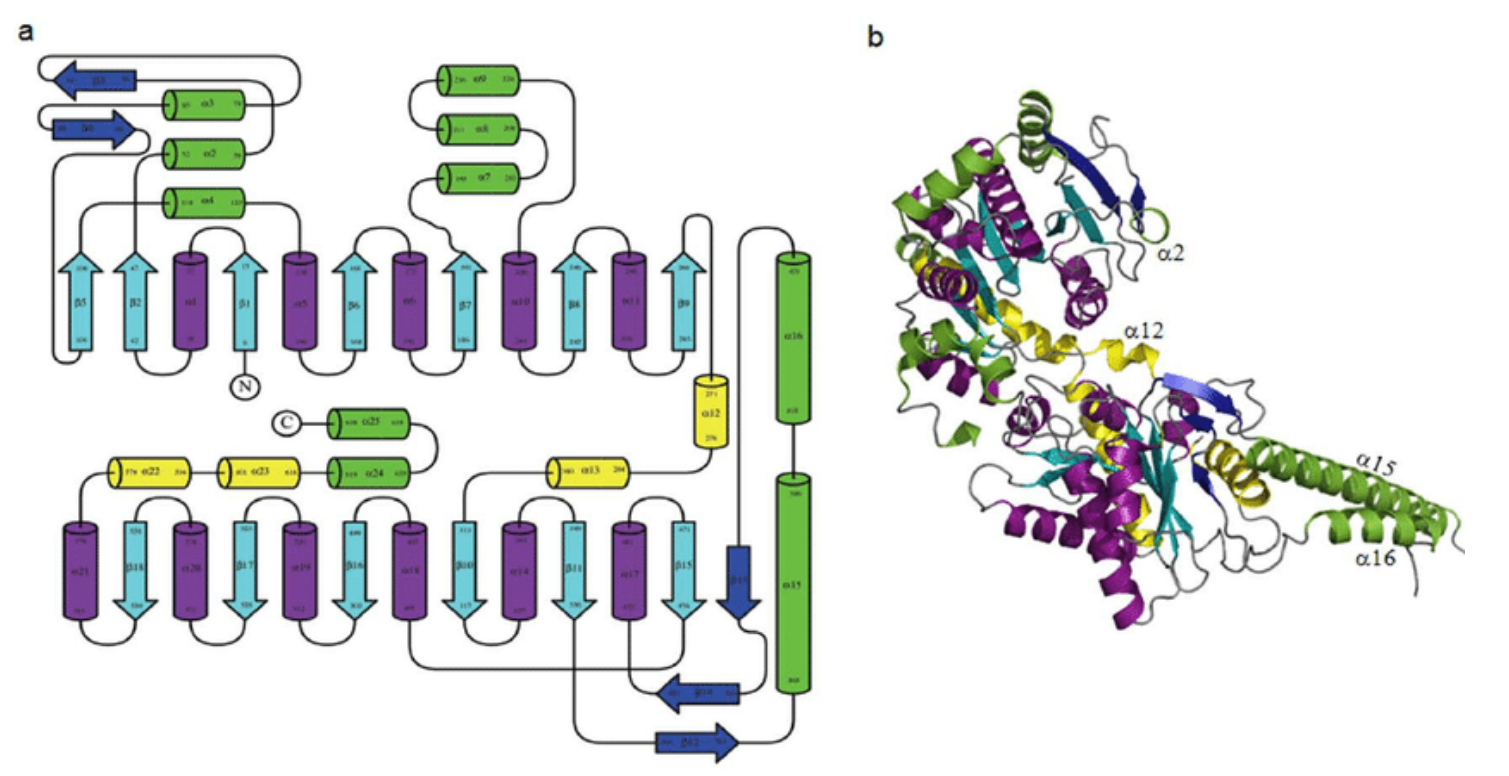
\includegraphics[width=\textwidth]{topology.png}
			\caption{The topology of a protein structure is a highly simplified description of its fold including only the sequence of secondary structure elements, and their relative spatial positions and approximate orientations. This information can be embodied in a two-dimensional diagram of protein topology, called a TOPS cartoon. (from pubmed)}
			\label{fig:topology}
			\end{figure}


\section{Coordinates}
The coordinates of all atoms in a protein are described in a PDB file.
This is a tabulated file containing different columns:

\begin{multicols}{2}
	\begin{itemize}
		\item Atom record: ATOM.
		\item Atom number: a unique identifier for the atom.
		\item Atom identifier: an identifier for the type of atom.
		\item Amino type: the amino acid from which the atom is from.
		\item Chain identifier: identifier for the chain.
		\item Residue sequence number: the number of the residue in the chain.
		\item $x$, $y$, $z$: the coordinates in angstrom.
		\item Occupancy: the probability of an atom to be in that space (confidence space).
		\item B-factor: how mobile that atom is in the crystal, it represent the noise in the x-ray diffraction map (it represents the fluctuations for the coordinate of the atoms. For example, loops in trans-membrane proteins are very mobile and a high B-factor is to be expected).
		\item Element symbol: the symbol of the element of the atom.
	\end{itemize}
\end{multicols}

Once the coordinates of a protein is obtained, some geometrical properties can be directly computed.

	\subsection{Protein centre of mass}
	The protein centre of mass is the average position for the protein centre.
	It is an average weighted by the mass of the atom.

	$$\vec{R}_{cm} = \frac{\sum\limits_{i=1}^Nm_i\vec{r}_i}{\sum\limits_{i=1}^Nm_i}$$

	\subsection{Radius of gyration}
	Once the centre of mass is known the radius of gyration can be computed.
	This measures the size of the protein as if it was a sphere.
	It is a good indication of the globular size of a protein.
	It also indicates an elongating/shrinking behaviour, and useful to check whether a protein is going toward equilibrium in the simulation.
	The distance of each atom and the centre of mass is computed and the square is taken, weighted with the mass of the atom.

	$$R_g = \sqrt{\frac{\sum\limits_{i=1}^Nm_i(\vec{r}_i-\vec{R}_{cm})^2}{\sum\limits_{i=1}^Nm_i}}$$

	\subsection{Comparing protein structures}
	Proteins have structures that loop in a similar way, with similar regions within each other.
	To quantify the similarity between the protein structure a procedure needs to be followed:

		\begin{itemize}
			\item Select common regions: a $1$-$1$ correspondence between amino acid need to be found: the parts present only in one protein are not considered.
				A correspondence is built between the common regions on the single amino-acids.
				These can be different, usually the coordinates are confronted between the $\alpha$-$C$ atom and the residue is not considered.
				One of the things that can be done is to look at the secondary structures and add loops only when they look similar.
			\item Align the two structures: compute the centre of mass of the two proteins and translate the proteins so the centre of masses coincide.
			\item Finding the optimal rotation: the principal axes are computed and the proteins are rotated so that they superimpose.
				Once the optimal rotation is obtained the difference can be quantified.
			\item Compute RMSD (root mean square deviation): take the coordinates of the amino-acid $i$ in protein $A$ and $B$, their squared difference is computed and an average over all amino acid is computed and squared:

				$$RMSD = \sqrt{\frac{1}{N}\sum\limits_{i=1}^N(\vec{r}_{Ai}-\vec{r}_{Bi})^2}$$
				the RMSD is a length, usually in angstrom scale.
				This can be done for two proteins or for the protein taken at two different time step in a molecular dynamics simulation:

				$$RMSD(t) = \sqrt{\frac{1}{N}\sum\limits_{i=1}^N(\vec{r}_{i}(t)-\vec{r}_{i}(0))^2}$$

				Now the $RMSD$ can be plotted with respect to time.
				It can be seen how at $t=0$ $RMSD=0$ and after the value will increase.
				When the number reaches a plateau the protein should be in equilibrium.
				The plateau can jump to another value, meaning that the state is a meta-stable state of the protein, or the protein has more stable states or a loop is making something.
				This value is assigned to very complicated structures and different structures can have the same $RMSD$.
				Clearly, a reference structure needs to be picked.
				In MD of a protein evolving in time, the reference structure is the initial configuration of the protein.
				One can also decide to focus on a specific region.
				The $RMSD$ is an indicator of equilibrium: it is a necessary but not sufficient condition.
		\end{itemize}

		\begin{figure}[H]
			\centering
			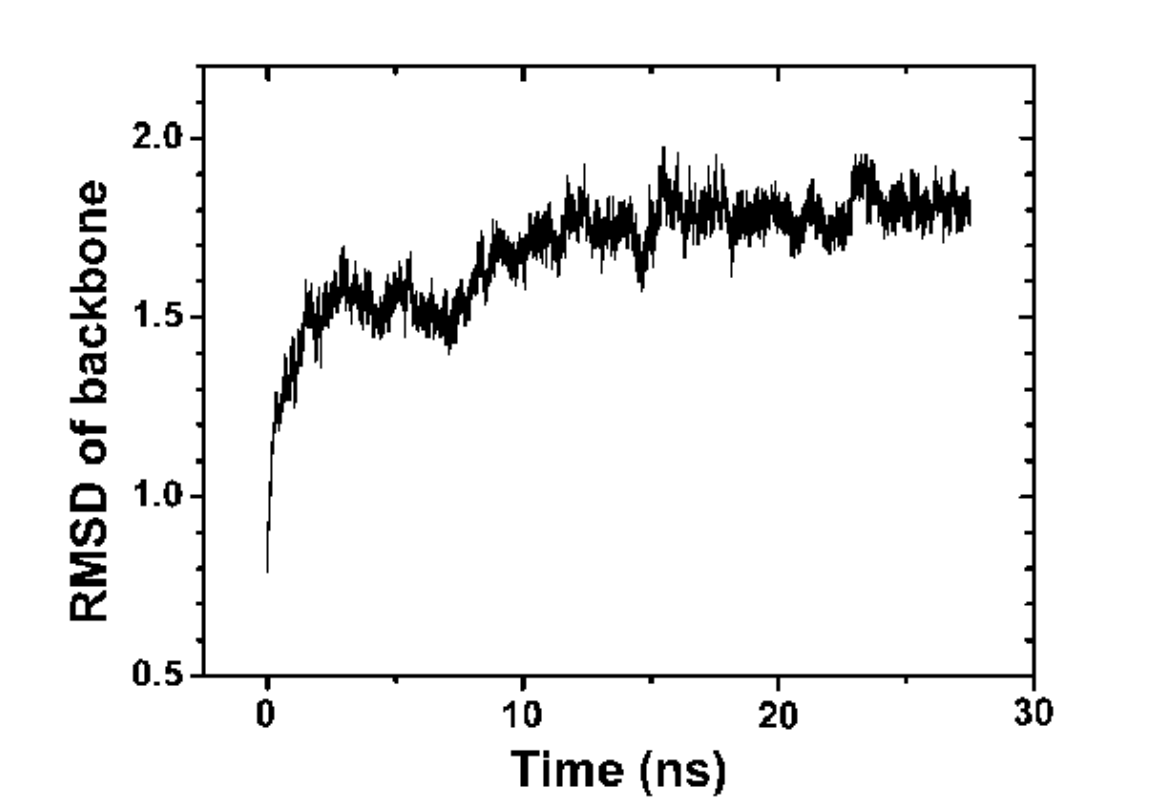
\includegraphics[scale = 0.3]{rmsd.png}
			\caption{RMSD of the backbone ($C^{\alpha}$, $N$, ...). We can see the typical steep jump a fluctuations towards the end of the plot. However, this is not enough to state that the protein reached equilibrium.}
			\label{fig:rmsd}
			\end{figure}


	\subsection{Native state}
	The native state is the functional state of a protein.
	It is not the state found for a crystallized protein, but only closely related to it, it is rather an ensemble in space and time of structures.
	This is due to proximity effect and the fact that the protein is not a static system.
	Proteins are extremely flexible and are moving a lot because the temperature corresponds to a constant movement of water molecule around causes movement in the protein.
	The native state is an ensemble of closely related states, all compatible with the conditions of the situation studied.
	Proteins need to be studied in the isothermal-isobaric ensemble.
	All the calculation need to be done at constant temperature and pressure.
	The native state is so a collection of functional state.

	In the case of the unfolded state the possibilities are too many to sample all of them.

	\subsection{RMSF}
	The flexibility of each amino acid can be computed.
	With flexibility is intended the movement of amino acid with respect to one another.
	In the $\alpha$-helix, for example, less fluctuation is expected, while in loops more fluctuation is expected.
	This quantity is computed in the root mean squared fluctuation, which will be computed for each amino acid in the protein.
	With $f$ referring to the frame, let:

	\begin{itemize}
		\item $\langle \vec{r}_i\rangle = \frac{1}{M}\sum\limits_{f=1}^M\vec{r}_{i,f}$, the average position of atom $i$.
		\item $\Delta\vec{r}_{i,f} = \vec{r}_{i,f}-\langle\vec{r}_i\rangle$, the displacement of each atom in each frame with respect to its average.
		\item $\langle \Delta\vec{r}_o^w\rangle = \frac{1}{M}\sum\limits_{f=1}^M(\vec{r}_{i,f}-\langle\vec{r}_i\rangle)^2$, the average squared distance over the frames.
	\end{itemize}

	So, the root mean squared fluctuation is:

	$$RMSF_i = \sqrt{\langle\Delta\vec{r}_i\rangle^2}$$

	Plotting the $RMSF$ with respect to residue number and the more mobile residue can be identified.
	This can be mapped onto the sequence so loops, helices and strands can be recognized.
	Usually the fluctuating part correspond to loops.
	The terminus have the highest $RMSF$.

		\subsubsection{B-factors}
		$RMSF$ can be translated into B-factors.
		They are the Debye-Waller factors and are a scaled version of the $RMSF$ squared.
		So the result of a simulation can be compared with the B-factor and a strong correspondence can be seen.
		The differences are due to the fact that the crystal is a different environment with respect to the normal one and packing effect can happen (some regions of the protein can interact with the image of the protein in the crystal).

		$$B_i = \frac{8\pi^2}{3}\langle\Delta\vec{r}_i^2\rangle = \frac{8\pi^2}{3}RMSF^2_i$$
